\documentclass[11pt]{amsart}
\usepackage[a4paper,margin=2.7cm]{geometry}
\usepackage{amssymb}
\usepackage{tikz}
\usepackage[hidelinks]{hyperref}

\newtheorem{theorem}{Theorem}
\newtheorem{lemma}{Lemma}
\newtheorem{corollary}[theorem]{Corollary}
\theoremstyle{remark}
\newtheorem{remark}{Remark}
\newtheorem{example}{Example}

\title[The Frobenius number of Dao's cyclic semigroups]{The Frobenius number of Dao's cyclic semigroups}
\author{Vamshi Jandhyala}
\date{Preprint, version 1, 23 October 2026. Not peer reviewed.}
\subjclass[2020]{20M14, 11D07, 13A02}
\keywords{numerical semigroup, Frobenius number, Ap\'ery set, mixed radix, determinantal ideal}

\begin{document}

\begin{abstract}
For positive integers $a_1,\dots,a_n$ ($n\ge2$, indices read cyclically) put $x_i=1+a_i+a_ia_{i+1}+\dots+a_ia_{i+1}\cdots a_{i+n-2}$. In 2018 Hailong Dao asked whether the numerical semigroup $\langle x_1,\dots,x_n\rangle$, when its generators are coprime and minimal, has Frobenius number $(n-1)(a_1a_2\cdots a_n-1)$, a direct extension of the two-generator formula. We prove this for every coprime list. The formula also follows from a theorem of Goto, Kien, Matsuoka and Truong once the semigroup ring is known to be cut out by the $2\times2$ minors of a cyclic $2\times n$ matrix; that presentation has not been established for this family, and the proof here does not use it. The argument is elementary: one identity, $a_{i-1}x_i=x_{i-1}+N$ with $N=a_1\cdots a_n-1$, turns every representation into a mixed-radix numeral modulo $N$, and carrying digits describes each residue class of the semigroup exactly.
\end{abstract}

\maketitle

\noindent\emph{Status of this preprint.} This version has not yet been independently reviewed.

\section{Introduction}

Two coprime integers $u,v\ge2$ generate a numerical semigroup whose largest missing integer is $uv-u-v$. Write $u=a+1$ and $v=b+1$ and the formula becomes $ab-1$: the Frobenius number is one less than the product of the shifts. Dao~\cite{MO} asked on MathOverflow in 2018 whether this pattern survives with more generators, for a particular cyclic choice of generators that arose in his work on monomial curves~\cite{MO2}. The question had no answer for eight years. This note answers it.

\emph{A first case.} Take $(a_1,a_2,a_3)=(1,2,3)$. The recipe below gives the generators
\[
x_1=1+1+1\cdot2=4,\qquad x_2=1+2+2\cdot3=9,\qquad x_3=1+3+3\cdot1=7 .
\]
The integers not in $\langle4,7,9\rangle$ are $1,2,3,5,6,10$, so the Frobenius number is $10$. Dao's formula predicts $(n-1)(a_1a_2a_3-1)=2\cdot5=10$.

In general, fix $n\ge2$ and positive integers $a_1,\dots,a_n$, and read every index modulo $n$. Put
\[
x_i=1+\sum_{j=0}^{n-2}a_ia_{i+1}\cdots a_{i+j}\qquad(1\le i\le n),
\]
so $x_i$ is $1$ plus the $n-1$ products of consecutive $a$'s that start at $a_i$ and stop short of a full turn. Write $S=\langle x_1,\dots,x_n\rangle$ for the set of all sums $\sum\lambda_ix_i$ with $\lambda_i\in\mathbb Z_{\ge0}$, and
\[
P=a_1a_2\cdots a_n,\qquad N=P-1 .
\]
When $n=2$ the generators are $1+a_1$ and $1+a_2$, and $N=a_1a_2-1$ is the classical answer.

\begin{theorem}\label{thm:main}
If $\gcd(x_1,\dots,x_n)=1$, then $(n-1)N\notin S$ and every integer $m>(n-1)N$ lies in $S$. So the Frobenius number of $S$ is
\[
F(S)=(n-1)(a_1a_2\cdots a_n-1).
\]
\end{theorem}

Dao also assumed that the $x_i$ generate $S$ minimally. The proof does not need this. In every coprime case we computed (Remark~\ref{rem:minimal}) the generators were minimal anyway, so we do not claim the omission as a strengthening.

\subsection*{Prior work}
The family is the cyclic case of a class studied in commutative algebra. Identity~\eqref{eq:carry} below says that the monomials $X_{i-1}$ and $X_i^{a_{i-1}}$ differ in degree by the same amount $N$ for every $i$, so the $2\times2$ minors of
\[
M=\begin{pmatrix} X_2^{a_1} & X_3^{a_2} & \cdots & X_1^{a_n}\\ X_1 & X_2 & \cdots & X_n\end{pmatrix}
\]
are homogeneous and vanish on the monomial curve $t\mapsto(t^{x_1},\dots,t^{x_n})$. Goto, Kien, Matsuoka and Truong~\cite[Theorem~1.2]{GKMT} proved that if a minimally generated numerical semigroup has its defining ideal equal to the ideal of $2\times2$ minors of a matrix of this shape, then its pseudo-Frobenius numbers are $\alpha,2\alpha,\dots,(n-1)\alpha$, where $\alpha$ is the common degree difference; Kien and Matsuoka~\cite[Theorem~3]{KM} extended this to cyclic two-row matrices with arbitrary exponents in both rows, where the progression starts at a shift $h$. For Dao's semigroups $\alpha=N$, and Theorem~\ref{thm:main} would follow. What is missing is the presentation itself: we found no proof that the minors of $M$ generate the whole defining ideal for this family, and recent work on when such presentations hold~\cite{MT,K} reduces the question to numerical conditions without settling this case. For $n=3$, Herzog's theorem~\cite{He} gives a presentation by the $2\times2$ minors of some $2\times3$ matrix whenever the semigroup is not symmetric, but not necessarily by $M$. The proof below avoids the presentation and uses only arithmetic.

\section{The carry identity}

Multiply the sum defining $x_i$ by $a_{i-1}$. Each product $a_ia_{i+1}\cdots a_{i+j}$ becomes $a_{i-1}a_i\cdots a_{i+j}$, which is a term of $x_{i-1}$, and the last one becomes the full product $P$. The constant $1$ becomes $a_{i-1}$, also a term of $x_{i-1}$. Only the constant $1$ of $x_{i-1}$ is not produced, so
\begin{equation}\label{eq:carry}
a_{i-1}\,x_i=x_{i-1}+N\qquad(1\le i\le n).
\end{equation}
In words: $a_{i-1}$ copies of $x_i$ are worth exactly one copy of $x_{i-1}$ plus $N$. In the first case, $1\cdot9=4+5$, $2\cdot7=9+5$ and $3\cdot4=7+5$.

Summing~\eqref{eq:carry} over $i$, the $x_{i-1}$ on the right run over all generators once, giving
\begin{equation}\label{eq:sum}
\sum_{i=1}^n(a_{i-1}-1)\,x_i=nN .
\end{equation}
So the vector with $a_{i-1}-1$ copies of each $x_i$ is worth $n$ times $N$; for $(1,2,3)$ it is $0\cdot9+1\cdot7+2\cdot4=15$.

Two consequences. If $P=1$ then every $a_i=1$ and every $x_i=n\ge2$, which contradicts coprimality, so $N\ge1$. And by~\eqref{eq:carry} a common divisor of $x_n$ and $N$ divides $x_{n-1}=a_{n-1}x_n-N$, then $x_{n-2}$, and so on round to $x_1$. Hence
\begin{equation}\label{eq:coprime}
\gcd(x_n,N)=1 .
\end{equation}

\section{Digit vectors}

Read~\eqref{eq:carry} modulo $N$: it says $x_{i-1}\equiv a_{i-1}x_i$, and iterating from $x_n$,
\begin{equation}\label{eq:place}
x_i\equiv\pi_i\,x_n\pmod N,\qquad \pi_i=a_ia_{i+1}\cdots a_{n-1}\ (1\le i<n),\quad\pi_n=1 .
\end{equation}
So modulo $N$ each generator is a fixed multiple of $x_n$, and a sum $\sum d_ix_i$ is $x_n$ times the number $\sum d_i\pi_i$. That number looks like a numeral with place values $\pi_i$, and it is one when each digit stays below its radix. This motivates the following definition. Call $d=(d_1,\dots,d_n)$ a \emph{digit vector} if $0\le d_i\le a_{i-1}-1$ for each $i$, and write $w(d)=\sum d_ix_i$ for its value.

So $w(d)\equiv x_n\sum_id_i\pi_i$, and $\sum_id_i\pi_i$ is an ordinary mixed-radix numeral: its place values are $\pi_n=1,\pi_{n-1}=a_{n-1},\pi_{n-2}=a_{n-2}a_{n-1},\dots,\pi_1$, and the digit in place $\pi_i$ runs below $a_{i-1}$ (the place $\pi_1$ has radix $a_n$, and $\pi_1a_n=P$). The standard facts about such numerals give the following lemma.

\begin{lemma}\label{lem:digits}
The numbers $\sum_id_i\pi_i$, as $d$ runs over digit vectors, are exactly $0,1,\dots,N$, each once. The value $0$ comes from $d=0$ and the value $N$ from the maximal vector $d_i=a_{i-1}-1$.
\end{lemma}

\begin{proof}
There are $\prod a_{i-1}=P=N+1$ digit vectors. Every integer $0\le t\le N$ has an expansion: divide by the radix of the lowest place, keep the remainder as the lowest digit, and repeat with the quotient. Two vectors with the same numeral agree in the lowest digit (both equal the remainder), and then in every digit by induction. The maximal vector gives $\sum(a_{i-1}-1)\pi_i=P-1$ because the sum telescopes.
\end{proof}

Combining the lemma with~\eqref{eq:coprime}: multiplication by $x_n$ permutes the residues modulo $N$, so the values $w(d)$ hit every nonzero residue class modulo $N$ exactly once, and the zero class twice, at $w(0)=0$ and at $w(\max)=nN$ by~\eqref{eq:sum}. Every digit vector has $w(d)\le nN$, again by~\eqref{eq:sum}. For $(1,2,3)$ the six digit vectors have values $0,4,8,7,11,15$, with residues $0,4,3,2,1,0$ modulo $5$.

\section{Proof of Theorem~\ref{thm:main}}

The plan is to describe, for each residue $r$ modulo $N$, the set $S\cap(r+N\mathbb Z)$. It turns out to be a ladder: a lowest rung at the digit value $w(d)$ in that class, then every rung $N$ apart above it. Moving down the ladder is carrying, moving up is uncarrying, and the Frobenius number is the highest missing rung, read off from~\eqref{eq:sum}. Figure~\ref{fig:ladders} shows the ladders for $(1,2,3)$.

\begin{figure}[ht]
\centering
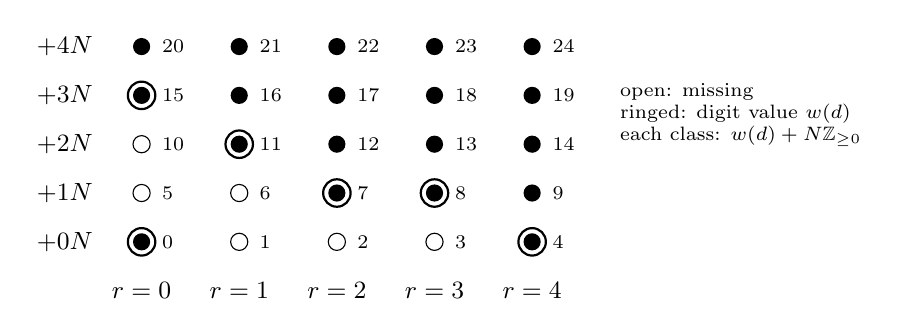
\begin{tikzpicture}[scale=0.62]
  \foreach \r in {0,...,4} { \node at (2*\r,-1) {\small $r=\r$}; }
  \foreach \k in {0,...,4} { \node[anchor=east] at (-0.8,\k) {\small $+\k N$}; }
  % members filled, gaps open; value = r + 5k
  \foreach \r/\k in {0/0,0/3,0/4, 1/2,1/3,1/4, 2/1,2/2,2/3,2/4, 3/1,3/2,3/3,3/4, 4/0,4/1,4/2,4/3,4/4}
     { \fill (2*\r,\k) circle (5pt); }
  \foreach \r/\k in {0/1,0/2, 1/0,1/1, 2/0, 3/0}
     { \draw (2*\r,\k) circle (5pt); }
  \foreach \r/\k/\v in {0/0/0,0/1/5,0/2/10,0/3/15,0/4/20,1/0/1,1/1/6,1/2/11,1/3/16,1/4/21,2/0/2,2/1/7,2/2/12,2/3/17,2/4/22,3/0/3,3/1/8,3/2/13,3/3/18,3/4/23,4/0/4,4/1/9,4/2/14,4/3/19,4/4/24}
     { \node[anchor=west,font=\scriptsize] at (2*\r+0.22,\k) {\v}; }
  % lowest rungs w(d)
  \foreach \r/\k in {0/0,0/3,1/2,2/1,3/1,4/0}
     { \draw[thick] (2*\r,\k) circle (8pt); }
  \node[anchor=west,font=\scriptsize,align=left] at (9.6,2.6) {open: missing\\ringed: digit value $w(d)$\\each class: $w(d)+N\mathbb Z_{\ge0}$};
\end{tikzpicture}
\caption{The residue classes modulo $N=5$ of $S=\langle4,9,7\rangle$, from $(a_1,a_2,a_3)=(1,2,3)$. Each column is a class; filled dots are elements of $S$. In each nonzero class the lowest element is the value of the unique digit vector in that class, and everything $N$ above it is in $S$. In the zero class the digit values are $0$ and $nN=15$, so $5$ and $10$ are missing and $10=(n-1)N$ is the Frobenius number.}
\label{fig:ladders}
\end{figure}

\emph{Carrying down.} Let $s=\sum\lambda_ix_i$ with $\lambda\ne0$. If some $\lambda_i\ge a_{i-1}$, replace $a_{i-1}$ copies of $x_i$ by one copy of $x_{i-1}$. By~\eqref{eq:carry} the value drops by exactly $N$, the residue modulo $N$ is unchanged, and the vector stays nonzero, since a copy of $x_{i-1}$ was added. The value cannot drop forever, so the process stops at a nonzero digit vector $d$ with
\begin{equation}\label{eq:down}
s=w(d)+kN\qquad\text{for some }k\ge0 .
\end{equation}

\emph{Carrying up.} Conversely, if $\lambda\ne0$ then some $\lambda_{i-1}\ge1$, and replacing one copy of $x_{i-1}$ by $a_{i-1}$ copies of $x_i$ raises the value by exactly $N$ and keeps the vector nonzero. Repeating, $w(d)+kN\in S$ for every nonzero digit vector $d$ and every $k\ge0$.

Together with Lemma~\ref{lem:digits} and~\eqref{eq:coprime} this gives the ladders. For a nonzero residue $r$ let $d(r)$ be the unique digit vector with $w(d(r))\equiv r$; then
\[
S\cap(r+N\mathbb Z)=\{\,w(d(r))+kN:\ k\ge0\,\}.
\]
In the zero class, a nonzero element of $S$ carries down to a nonzero digit vector with residue $0$, which must be the maximal vector, so
\[
S\cap N\mathbb Z=\{0\}\cup\{\,nN+kN:\ k\ge0\,\}.
\]
The first display reads: in class $r$ the members of $S$ are the digit value $w(d(r))$ and everything $N$ above it. The second reads: the multiples of $N$ in $S$ are $0$ and those from $nN$ upwards.

Now the Frobenius number. In a nonzero class the largest missing integer is $w(d(r))-N$, and $w(d(r))<nN$ because the value $nN$ belongs to the zero class; so it is at most $(n-1)N-1$. In the zero class the largest missing integer is $(n-1)N$, which is positive because $n\ge2$ and $N\ge1$. Hence $(n-1)N\notin S$ and every larger integer is in $S$. \qed

\section{Remarks and checks}

\begin{remark}\label{rem:minimal}
Dao's question assumed the $x_i$ generate $S$ minimally, and the proof above never uses it. We tested whether it can fail: in all $3{,}703$ coprime lists with $2\le n\le5$ and entries at most $8$ (for $n\le3$) or $5$ (for $n=4,5$), and $14{,}459$ random coprime lists with $n\le7$, no generator was a combination of the others. We have not proved that minimality always holds.
\end{remark}

\begin{remark}\label{rem:pf}
The theorem of Goto, Kien, Matsuoka and Truong predicts more than the Frobenius number: if the presentation by the minors of $M$ holds, the pseudo-Frobenius numbers of $S$ (the missing $f$ with $f+x_i\in S$ for every $i$) are exactly $N,2N,\dots,(n-1)N$. We computed them in $2{,}186$ random coprime cases with $n\le5$ and found exactly this set every time. The ladders above suggest a direct proof, which we have not written down.
\end{remark}

\emph{Verification.} The accompanying repository checks Theorem~\ref{thm:main} and the ladder description of every residue class against a brute-force computation for all $2{,}379$ coprime lists with $2\le n\le6$ and entries at most $8,8,5,4,3$ respectively. An independent program, sharing no code with the first, recomputes the same Frobenius numbers by shortest paths on residues modulo the smallest generator. Further scripts reproduce the worked example and the counts in the remarks. The whole proof of Theorem~\ref{thm:main}, including Lemma~\ref{lem:digits} and the carrying arguments, is formalised in Lean~4 with Mathlib, following the steps above.

\emph{Acknowledgement.} The proof was developed with the help of Claude (Anthropic) and ChatGPT (OpenAI). Claude drafted this note and the Lean formalisation. The question is due to Hailong Dao.

\begin{thebibliography}{9}
\bibitem{GKMT} S.~Goto, D.~V.~Kien, N.~Matsuoka and H.~L.~Truong, Pseudo-Frobenius numbers versus defining ideals in numerical semigroup rings, \emph{J.~Algebra} \textbf{508} (2018), 1--15. arXiv:1705.06902.
\bibitem{He} J.~Herzog, Generators and relations of abelian semigroups and semigroup rings, \emph{Manuscripta Math.} \textbf{3} (1970), 175--193.
\bibitem{K} D.~V.~Kien, Arithmetic pseudo-Frobenius numbers and determinantal numerical semigroup rings, arXiv:2609.39218 (2026).
\bibitem{KM} D.~V.~Kien and N.~Matsuoka, Numerical semigroup rings of maximal embedding dimension with determinantal defining ideals, in \emph{Numerical Semigroups}, Springer INdAM Ser.~\textbf{40}, Springer, 2020, 185--196.
\bibitem{MO} H.~Dao, A formula for Frobenius number of certain numerical semigroups, MathOverflow question 292507 (2018), \url{https://mathoverflow.net/q/292507}, accessed 23 October 2026.
\bibitem{MO2} H.~Dao, answer to ``Square of primary ideals'', MathOverflow question 149713 (2017), \url{https://mathoverflow.net/q/149713}, accessed 23 October 2026.
\bibitem{MT} S.~Murai and K.~Takahashi, A criterion for determinantal presentations of numerical semigroup rings, arXiv:2609.18136 (2026).
\end{thebibliography}

\end{document}
